\documentclass[11pt]{article}

\usepackage{graphics} % or graphicx 
\usepackage{epstopdf}
\usepackage{multirow}
\usepackage{amsmath}
\usepackage{bbding}
\usepackage{pifont}
\usepackage{wasysym}
\usepackage{amssymb}
\usepackage{subcaption}

%%\usepackage[parfill]{parskip}



\setlength{\oddsidemargin}{0in}
\setlength{\textwidth}{6.5in}
\setlength{\topmargin}{-0.5in}
\setlength{\textheight}{8.75in}
\setlength{\parindent}{0pt}
\setlength{\parskip}{6pt}

\usepackage{fancyhdr}
\pagestyle{fancy}
\lhead{HW4}
\rhead{Reza Shisheie}

\usepackage{epsfig,graphicx}

\usepackage{amsmath}

\usepackage{clrscode3e}

\begin{document}

\thispagestyle{plain}

\begin{center}
{\Large \bf CIS 606 \hfil Homework 4 \hfil Fall 2019} \\
\end{center}

\vskip 1in 

\centerline{
\includegraphics[width=3in]{photo.jpg}}

\vskip 0.5in 


\begin{center}
\begin{tabular}{ll}
{\bf Name:}     & {\bf Reza Shisheie } \\ \\
{\bf Login ID:} & {\bf reshishe }   
\end{tabular}
\end{center}

\newpage

\begin{enumerate}

\itemsep 0.35in


\item Exercise 5.2-b (Textbook page 144): Suppose that there is exactly one index $i$ such that $A[i] =x$. What is the expected number of indices into A that we must pick before we find $x$ and RANDOM-SEARCH terminates?
	
	In each iteration:
	
	\hspace{10mm} $P(\mathrm{A}[i]=x) = \frac{1}{n}$
	
	\hspace{10mm} $P(\mathrm{A}[i]\neq x) = \frac{n-1}{n}$

	From induction:
	
	$i=1$: Finding $x$ in  1st shot:
	
	\hspace{10mm} $E(s,i=1) = \frac{1}{n}$. 

	$i=2$: Finding $x$ in 1st shot + 2nd shot:
	
	\hspace{10mm} $E(s,i=2) = (\frac{1}{n})\cdot(1-\frac{1}{n}) + (1-\frac{1}{n}) \cdot (\frac{1}{n}) =
				\frac{n-1}{n} \cdot \frac{2}{n} $
		
	$i=3$: Finding $x$ in 1st shot + 2nd shot + 3rd shot:
	
	\hspace{10mm} $E(s,i=3) =  (\frac{1}{n}) \cdot (1-\frac{1}{n}) \cdot (1-\frac{1}{n})  + (1-\frac{1}{n}) \cdot (\frac{1}{n}) \cdot (1-\frac{1}{n}) + (1-\frac{1}{n}) \cdot (1-\frac{1}{n}) \cdot (\frac{1}{n}) = 
	(\frac{n-1}{n})^{2} \cdot \frac{3}{n} $

	
	Doing it $i$ ietrations:
	
	\hspace{10mm} $E(s,i) = \sum_{i=1}^{\infty} (\frac{n-1}{n})^{i-1}\cdot\frac{i}{n}=
	 \frac{1}{n-1} \cdot \sum_{i=1}^{\infty} (\frac{n-1}{n})^{i}\cdot i= 
	 \frac{1}{n-1} \cdot \sum_{i=0}^{\infty} (\frac{n-1}{n})^{i}\cdot i$
	
	From CLRS.A.8, page 1148:
	
	\hspace{10mm} $\sum_{k=0}^{\infty} k\cdot x^{k}=\frac{x}{(1-x)^{2}}$, if $|x|<1$	
	
	Knowing $|\frac{n-1}{n}|<1$, thus:
	
	\hspace{10mm} $E(s,i) = \frac{1}{n-1} \cdot \sum_{i=0}^{\infty} (\frac{n-1}{n})^{i}\cdot i = 
	\frac{1}{n-1} \cdot \frac{\frac{n-1}{n}}{(1-\frac{n-1}{n})^{2}} = 
	\frac{1}{n-1} \cdot \frac{\frac{n-1}{n}}{\frac{1}{n^{2}}}=n$
	 
	
	

\item Exercise 5.2-c (Textbook page 144): Generalizing your solution to part (b), suppose that there are $k\geq 1$ indices $i$ such that $A[i]=x$. What is the expected number of indices into $A$ that we must pick before we find $x$ and RANDOM-SEARCH terminates? Your answer should be a function of $n$ and $k$.

	Generalizing previous example to a ranges of indecies $k>1$: 

	\hspace{10mm} $P(\mathrm{A}[i]=x) = \frac{k}{n}$
	
	\hspace{10mm} $P(\mathrm{A}[i]\neq x) = \frac{n-k}{n}$
	
	Now repeating for $i$ ietrations:
	
	\hspace{10mm} $E(s,i) = \sum_{i=1}^{\infty} (\frac{n-k}{n})^{i-1}\cdot\frac{k}{n}\cdot i=
	 \frac{k}{n-k} \cdot \sum_{i=1}^{\infty} (\frac{n-k}{n})^{i}\cdot i= 
	 \frac{k}{n-k} \cdot \sum_{i=0}^{\infty} (\frac{n-k}{n})^{i}\cdot i$
	 
 	From CLRS.A.8, page 1148:
	
	\hspace{10mm} $\sum_{k=0}^{\infty} k\cdot x^{k}=\frac{x}{(1-x)^{2}}$, if $|x|<1$	
	
	Knowing $|\frac{n-k}{n}|<1$, thus:

	\hspace{10mm} $E(s,i) = \frac{k}{n-k} \cdot \sum_{i=0}^{\infty} (\frac{n-k}{n})^{i}\cdot i = 
	\frac{k}{n-k} \cdot \frac{\frac{n-k}{n}}{(1-\frac{n-k}{n})^{2}} = 
	\frac{k}{n-k} \cdot \frac{\frac{n-k}{n}}{\frac{k^{2}}{n^{2}}}=\frac{n}{k}$


\pagebreak
\item Exercise 6.3-1 (Textbook page 159) draw like Figure 6.3: Using Figure 6.3 as a model, illustrate the operation of BUILD-MAX-HEAP on the
array $A=\langle 5, 3, 17, 10, 84, 19, 6, 22, 9 \rangle	$.

	As heap $A$ has 9 elements then the starting element will be START = 
	$\lfloor	 \frac{9}{2}	\rfloor	 = 4$

	Figure.\ref{fig:prob-6-3-1} shows the start point:

	\begin{figure}[!h]

		\begin{subfigure}{.5\textwidth}
			\centerline{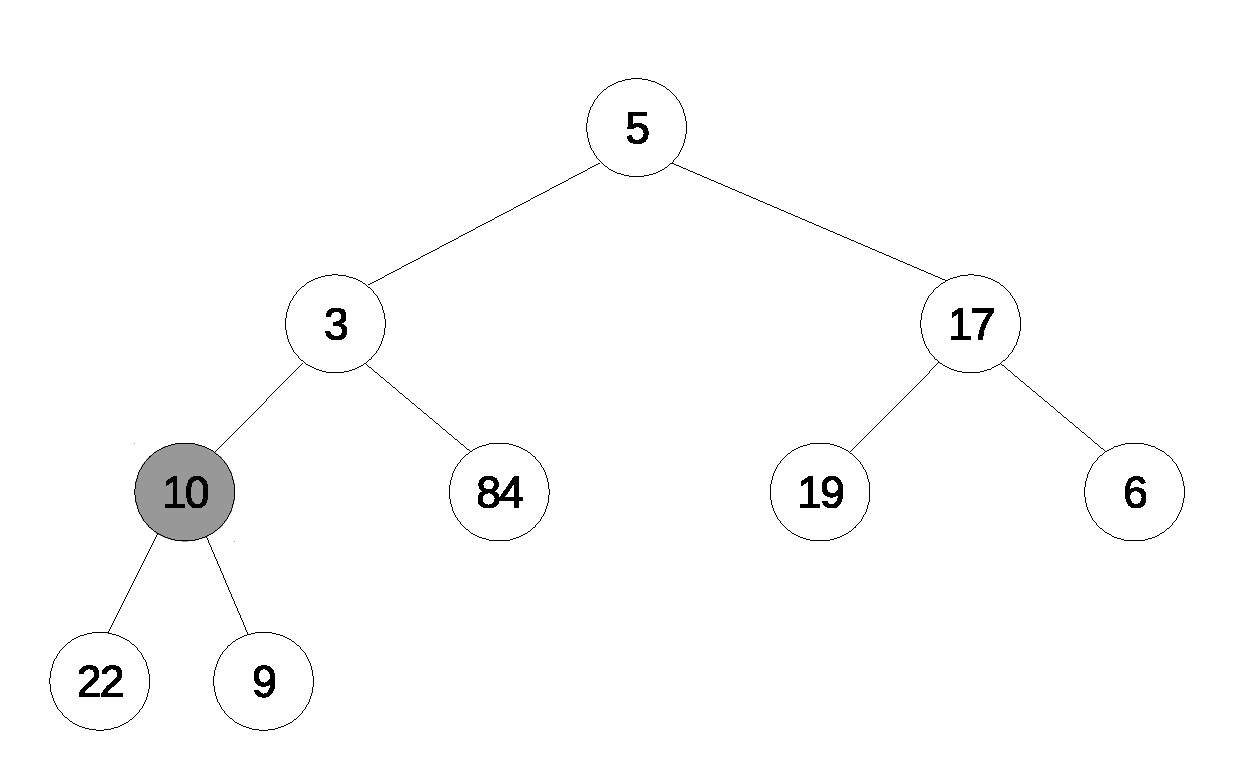
\includegraphics[width=2.5in]{prob-6-3-1_1.eps}}
			\caption{Starting point}
			\label{fig:prob-6-3-1_1}
		\end{subfigure}%
		\begin{subfigure}{.5\textwidth}
			\centerline{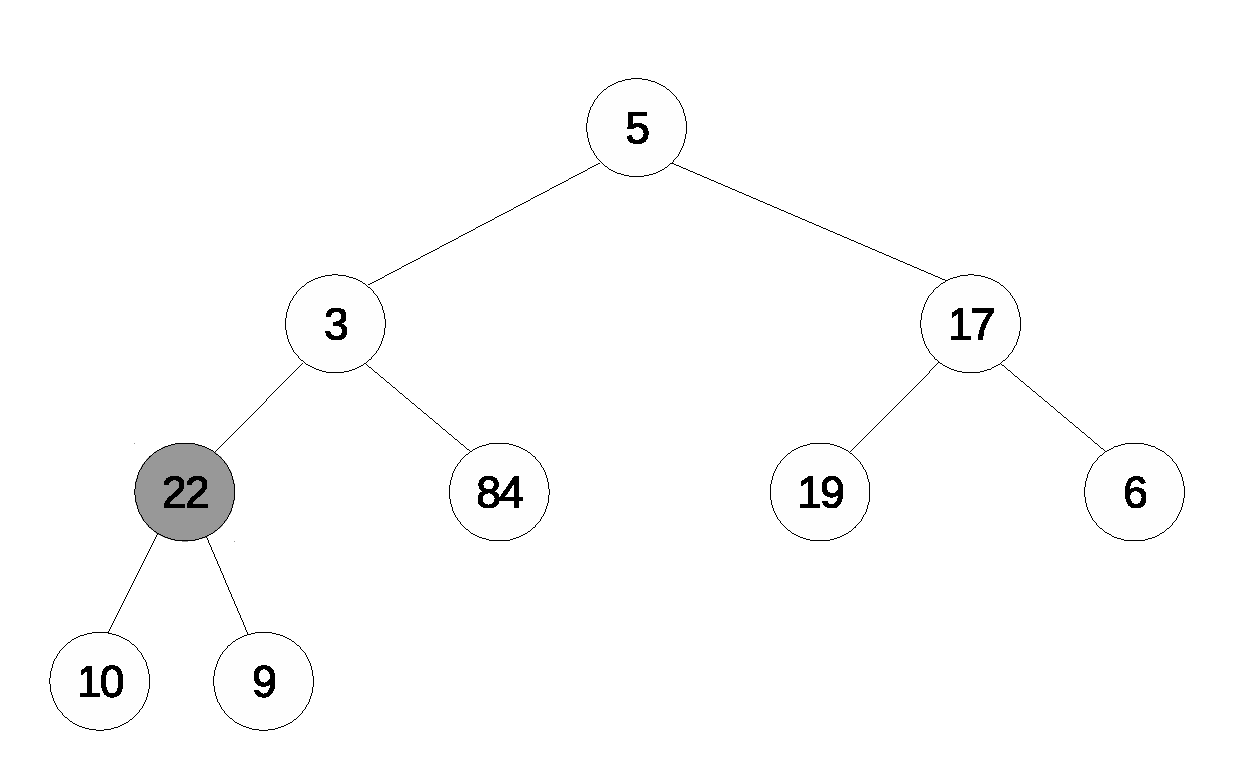
\includegraphics[width=2.5in]{prob-6-3-1_2.eps}}
			\caption{After 1st iteration of BUILD-MAX-HEAP}
			\label{fig:prob-6-3-1_2}
		\end{subfigure}
		
		\begin{subfigure}{.5\textwidth}
			\centerline{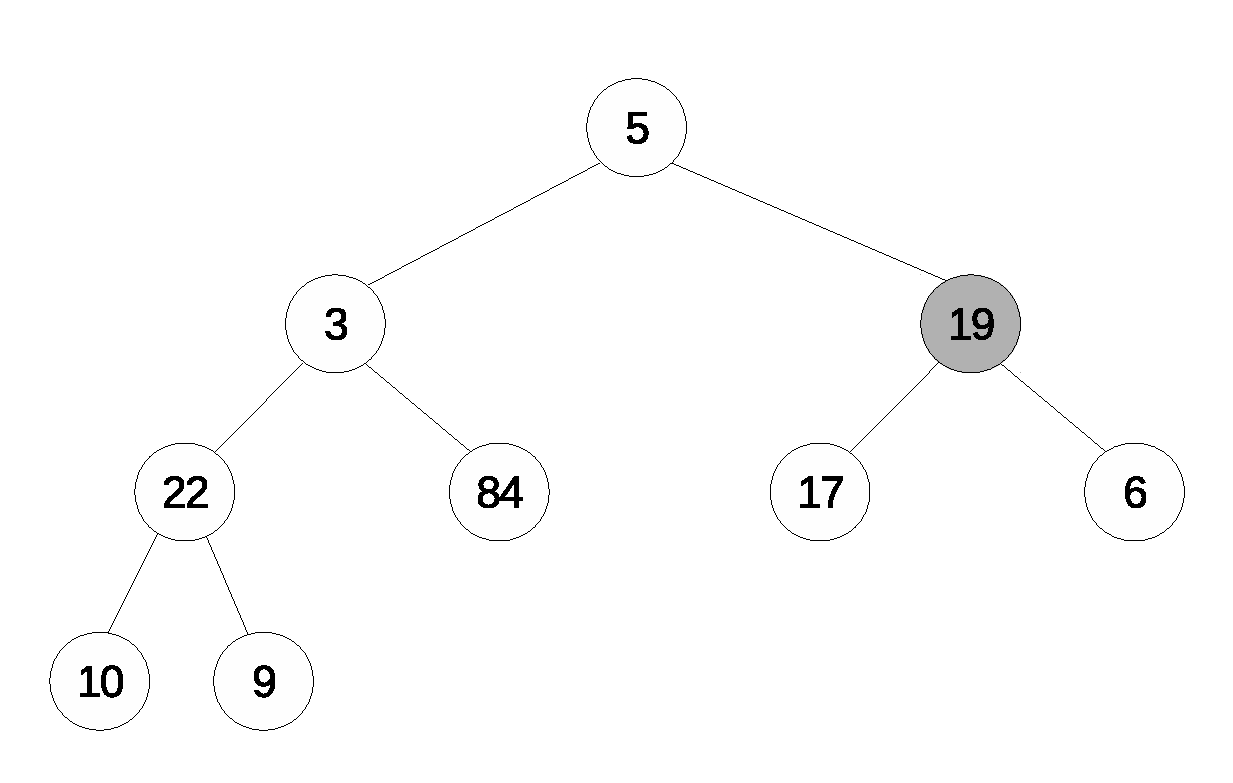
\includegraphics[width=2.5in]{prob-6-3-1_3.eps}}
			\caption{After 2nd iteration of BUILD-MAX-HEAP}
			\label{fig:prob-6-3-1_3}
		\end{subfigure}%		
		\begin{subfigure}{.5\textwidth}
			\centerline{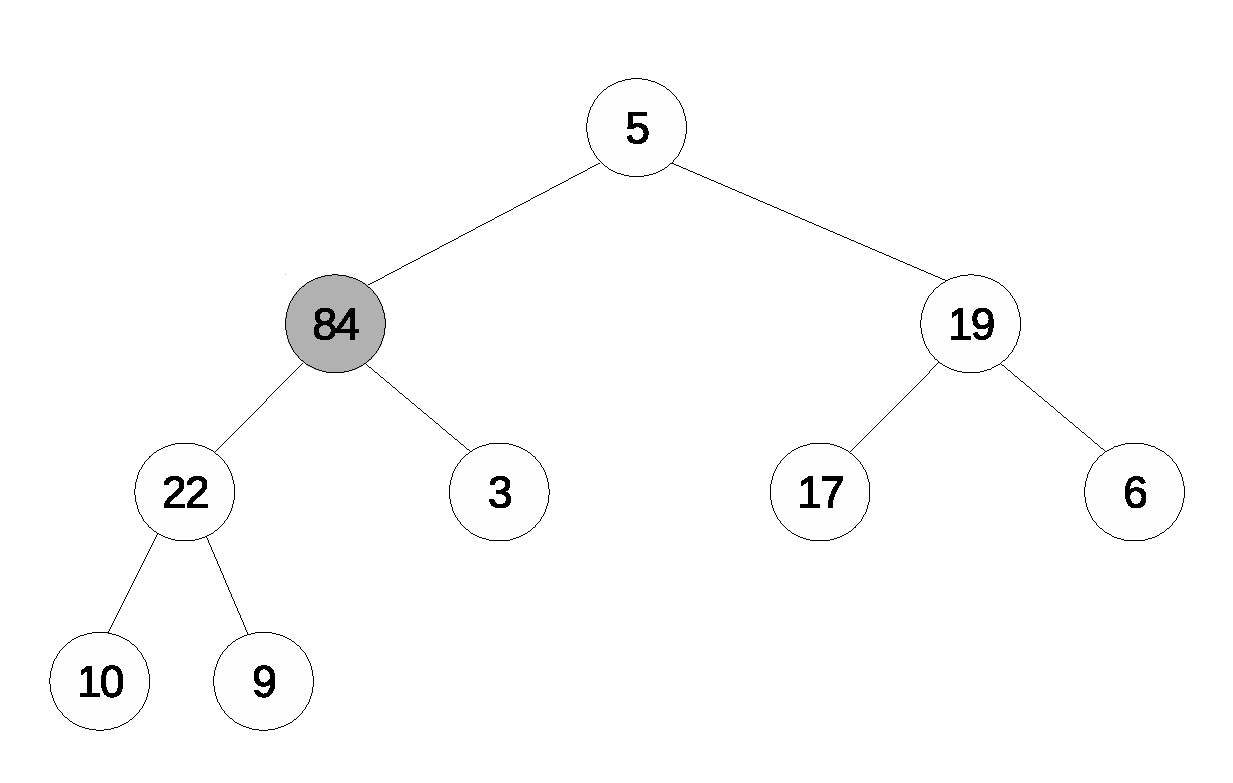
\includegraphics[width=2.5in]{prob-6-3-1_4.eps}}
			\caption{After 3rd iteration of BUILD-MAX-HEAP}
			\label{fig:prob-6-3-1_4}
		\end{subfigure}
				
		\begin{subfigure}{.5\textwidth}
			\centerline{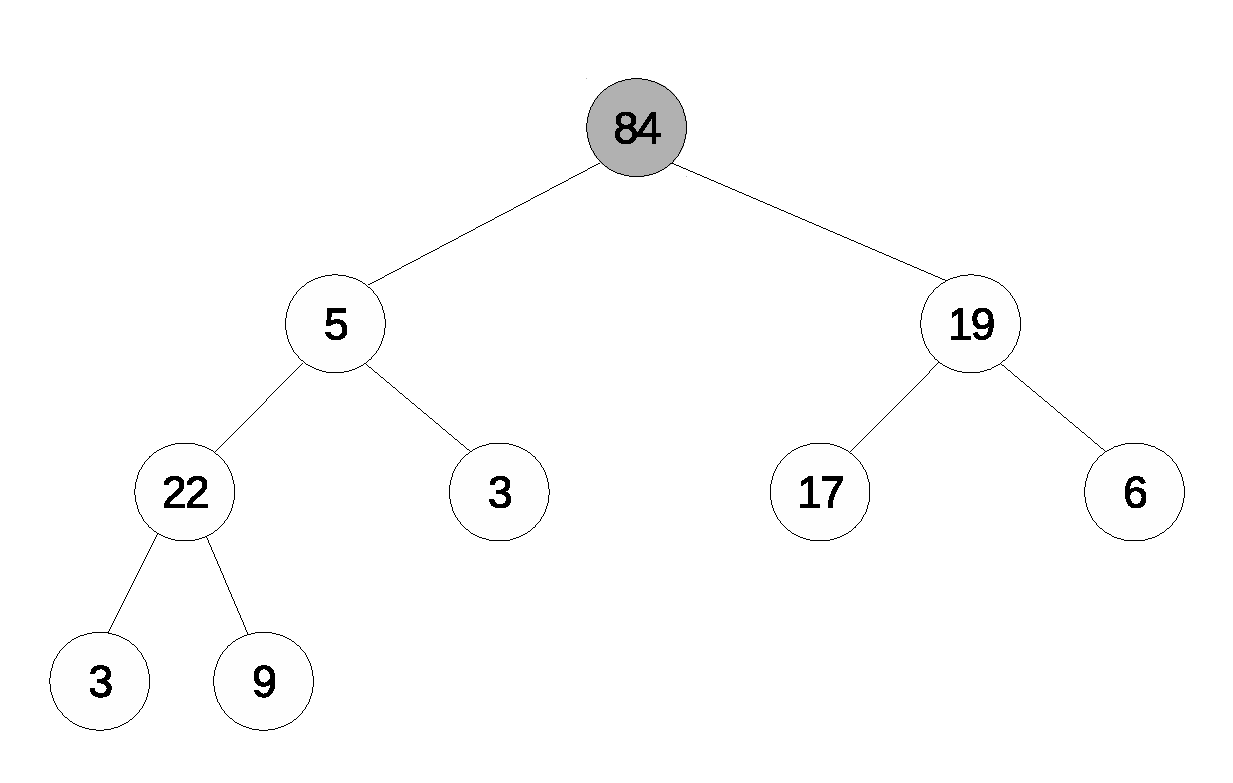
\includegraphics[width=2.5in]{prob-6-3-1_5.eps}}
			\caption{After 4th iteration of BUILD-MAX-HEAP}
			\label{fig:prob-6-3-1_5}
		\end{subfigure}%		
		\begin{subfigure}{.5\textwidth}
			\centerline{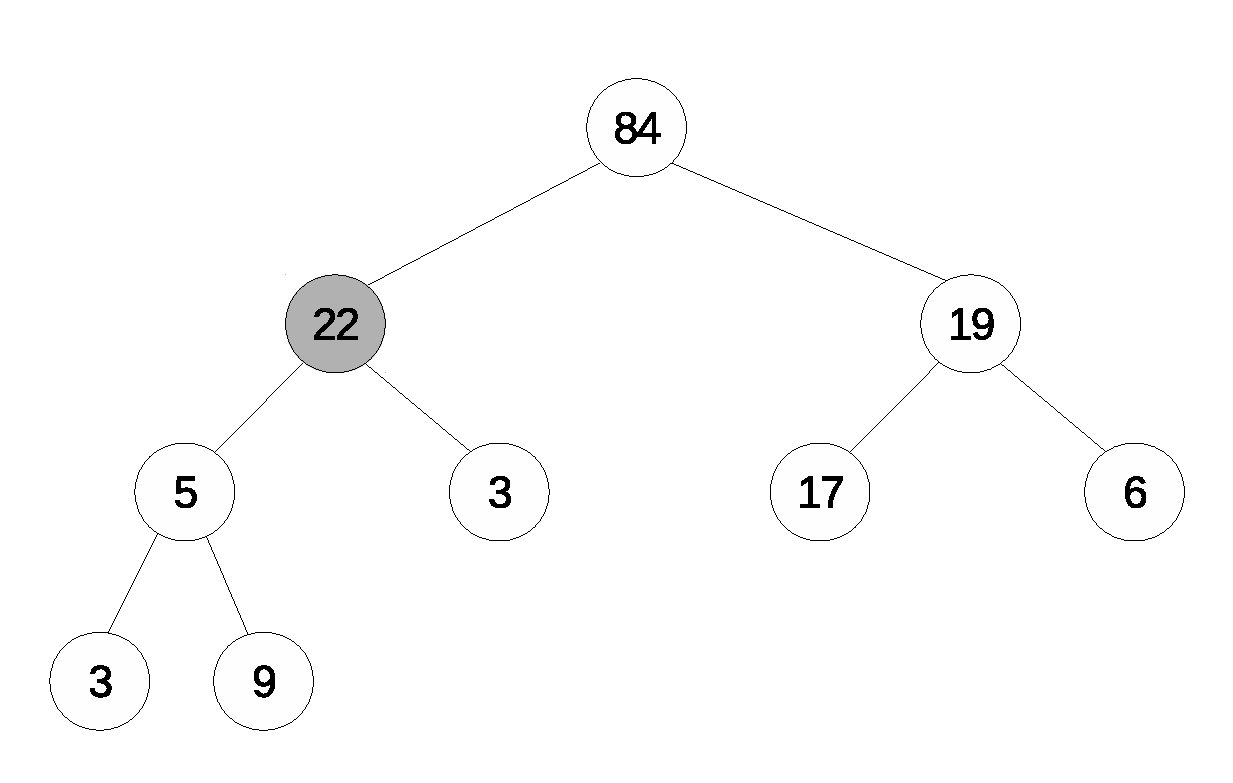
\includegraphics[width=2.5in]{prob-6-3-1_6.eps}}
			\caption{After 5th iteration of BUILD-MAX-HEAP}
			\label{fig:prob-6-3-1_6}
		\end{subfigure}
		
		\begin{subfigure}{.5\textwidth}
			\centerline{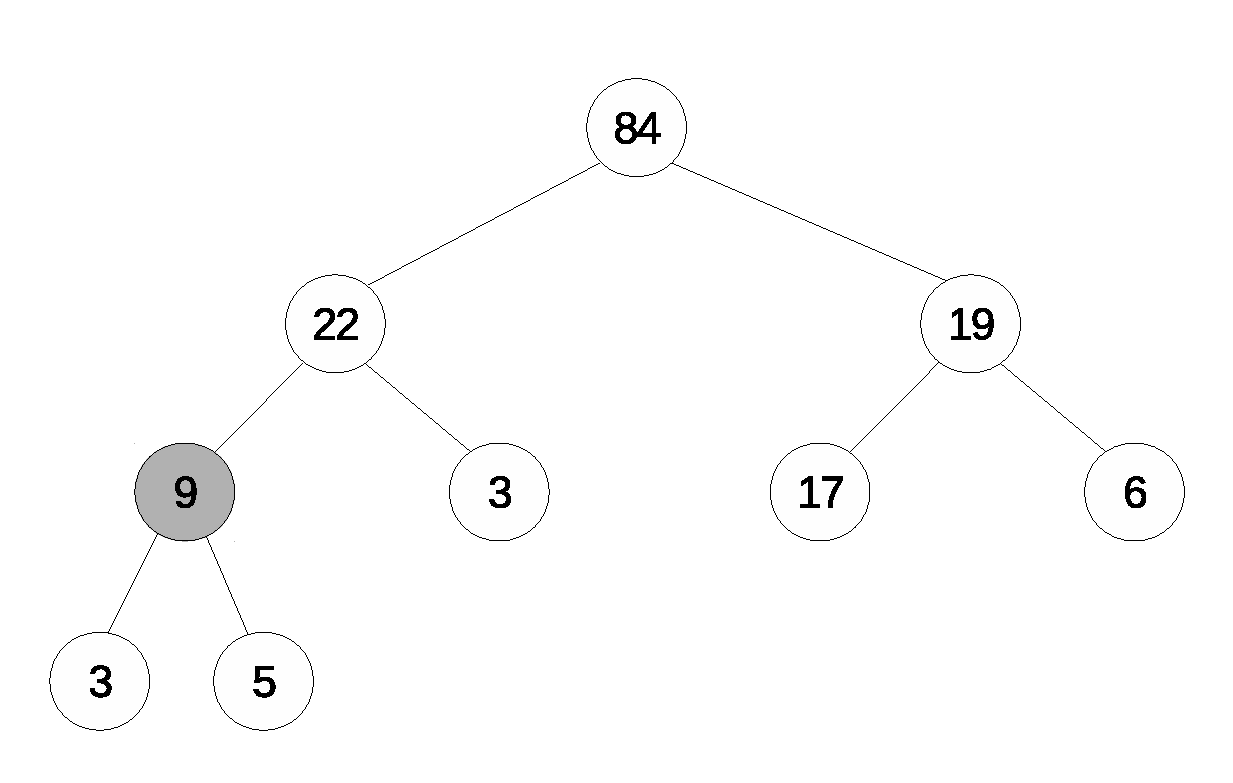
\includegraphics[width=2.5in]{prob-6-3-1_7.eps}}
			\caption{After 6th iteration of BUILD-MAX-HEAP}
			\label{fig:prob-6-3-1_6}
		\end{subfigure}

		\caption{Iteration of BUILD-MAX-HEAP}
		\label{fig:prob-6-3-1}
	\end{figure}
	
	
\pagebreak
 
\item Exercise 6.5-9 (Textbook page 166): Give an $O(n\log{k})$-time algorithm to merge $k$ sorted lists into one sorted list, where $n$ is the total number of elements in all the input lists. ($Hint$: Use a min-heap for $k$-way merging.)

	
	Figure.\ref{fig:prob-6-5-9} shows the suggested min-heap structure to sort array $A$, assuming array $A[1...n]$ with $n$ elements is divided into $k$ sorted sub-arrays $a_{sorted}$: 

	\begin{figure}[h!]
		\centerline{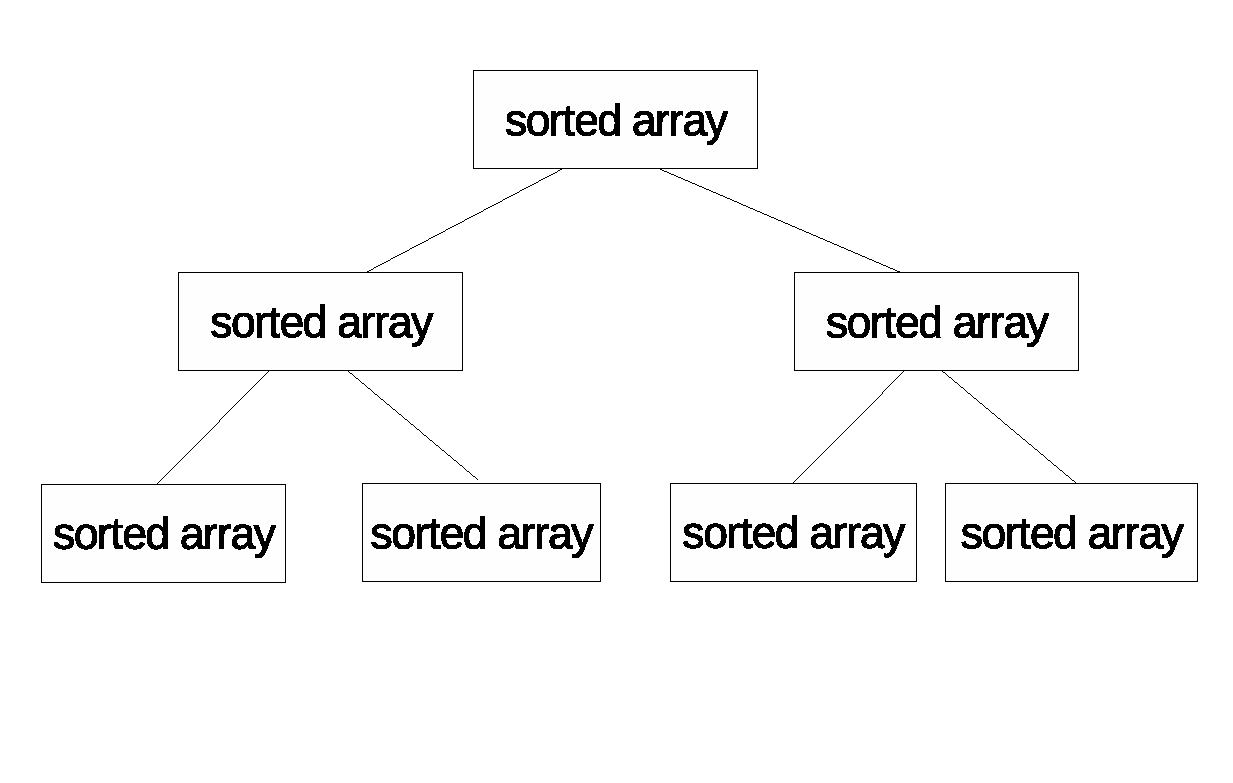
\includegraphics[width=4in]{prob-6-5-9.eps}}
		\caption{Structure of sorted array in min-heap}
		\label{fig:prob-6-5-9}
	\end{figure}
	
	In this structure, each $sorted$ $subarray$ is represented by its minimum element. Using the represnted minimum values of each subarray, a heap is generated. In this structure, the minimum element of the root $subarray$ is the global minimum in the heap.
	
	After each MIN-HEAP procedure, minimum value of the $subarray$ in the root is removed from heap, and replaced with the next element in the $subarray$. Now heap has to be adjusted with a new value at root (this is similar to inserting a new value to the root and min-heap).  	
	
	This algorithm is similar to min heap-sort algorithm. Based on the proof provided in CLRS p.163, time complexity of HEAP-EXTRACT-MAX with $k$ elements is $O(\log{k})$. Without loss of generality, time complexity of the HEAP-EXTRACT-MIN with $k$ elements is $O(\log{k})$ too. Every time HEAP-EXTRACT-MIN is implemented, only one element at the root $subarray$ is removed. Thus HEAP-EXTRACT-MIN has to get executed $n$ times. Therefore time complexity is $O(n\log{k})$   
	
	

	
	
	   




















































   
\end{enumerate}

\end{document}

